\documentclass[10pt]{dokument-ppi}

\begin{document}


\Cwiczenie{2}
\Tytul{Kontekst i opis produktu}
\Data{2012-12-27}
\Wersja{2.0}
\Autorzy{TC}
\MakeDokumentMeta


\section{Kontekst}

Kampus Politechniki Warszawskiej jest popularnym miejscem działań agencji
marketingowych promujących wydarzenia kulturowe, w szczególności koncerty. Wybór
miejsca jest podyktowany kilkoma czynnikami:
\begin{itemize}
    \item studenci są główną grupą docelową tego typu wydarzeń,
    \item kampus zapewnia duży przepływ osób z grupy docelowej,
    \item studenci są aktywnymi konsumentami kultury --- łatwo jest ich
        zaangażować w akcjach promocyjnych.
\end{itemize}
W efekcie, nie potrzeba wiele nakładów by wypromować koncert na kampusie
Politechniki Warszawskiej. Sprawdzoną i wystarczającą metodą promocji jest
wywieszenie plakatów promujących wydarzenie w widocznych miejscach, na przykład
przed wejściami do Gmachu Głównego. Tak umieszczony plakat wystarczy, by
przekonać pojedynczych studentów. Oni natomiast zaproszą osobiście swoich
znajomych. Jedynym problemem tego scenariusza jest zawodna pamięć studentów,
zwłaszcza gdy zobaczyli plakat biegnąc na wykład, by uniknąć spóźnienia.


% \section{Cel projektu}
%
% Celem projektu Concerto jest stworzenie systemu \emph{Software-as-a-Service}.
% Usługa jest oferowana organizatorom wydarzeń kulturalnych. Ma na celu
% zwiększenie skuteczności akcji reklamowych wykorzystujących plakaty poprzez:
% \begin{itemize}
%     \item ułatwienie kupna biletu na wydarzenie od organizatora wydarzenia,
%     \item wygodne przekazywanie zaproszeń na wydarzenie pomiędzy znajomymi,
%     \item szybki sposób dodania wydarzenia do kalendarza osoby bezpośrednio
%         zainteresowanej.
% \end{itemize}


\section{Opis produktu}

System Concerto składa się trzech komponentów:
\begin{enumerate}
    \item \textbf{aplikacja mobilna} dla adresatów akcji reklamowych,
    \item \textbf{serwer obsługi zapytań} aplikacji mobilnych,
    \item \textbf{API udostępniane organizatorom} do zarządzania informacjami o
        ich wydarzeniach kulturalnych.
\end{enumerate}
Schemat współpracy komponentów jest przedstawiony
na~stronie~\pageref{fig:schemat_komponentow}.

\subsection{Aplikacja mobilna}
Głównym celem aplikacji mobilnej jest dostarczenie użytkownikowi informacji o
wydarzeniu oraz zaproponowanie kupna biletu w sklepie internetowym organizatora.

Po uruchomieniu aplikacji użytkownik robi zdjęcie plakatu, który go
zainteresował. Aplikacja wysyła zdjęcie do serwera obsługi zapytań i oczekuje na
odpowiedź. Zwracane są podstawowe informacje, takie jak czas i miejsce
wydarzenia, cena biletu oraz propozycja zakupu biletu bezpośrednio w sklepie
internetowym organizatora.

Następnie umożliwia zaproszenie znajomych na wydarzenie korzystając z
popularnych sieci społecznościowych oraz standardowych środków komunikacji,
takich jak email czy SMS.

\subsection{Serwer obsługi zapytań}
Serwer obsługi zapytań jest dostępny przez połączenie internetowe. Serwer
posiada bazę danych z informacjami o wydarzeniach, w szczególności obrazy
plakatów wykorzystywanych w akcjach reklamowych. Po otrzymaniu zapytania,
serwer porównuje zdjęcie z plakatami z bazy i zwraca informacje przypisane do
plakatu.

\subsection{API zarządzania bazą wydarzeń}
System ściśle współpracujący z serwerem obsługi zapytań. Pozwala organizatorom
wydarzeń na zarządzanie plakatami i informacjami o wydarzeniach do serwera
obsługi zapytań.

\subsection{Współpraca komponentów}
\begin{figure}[h!]
    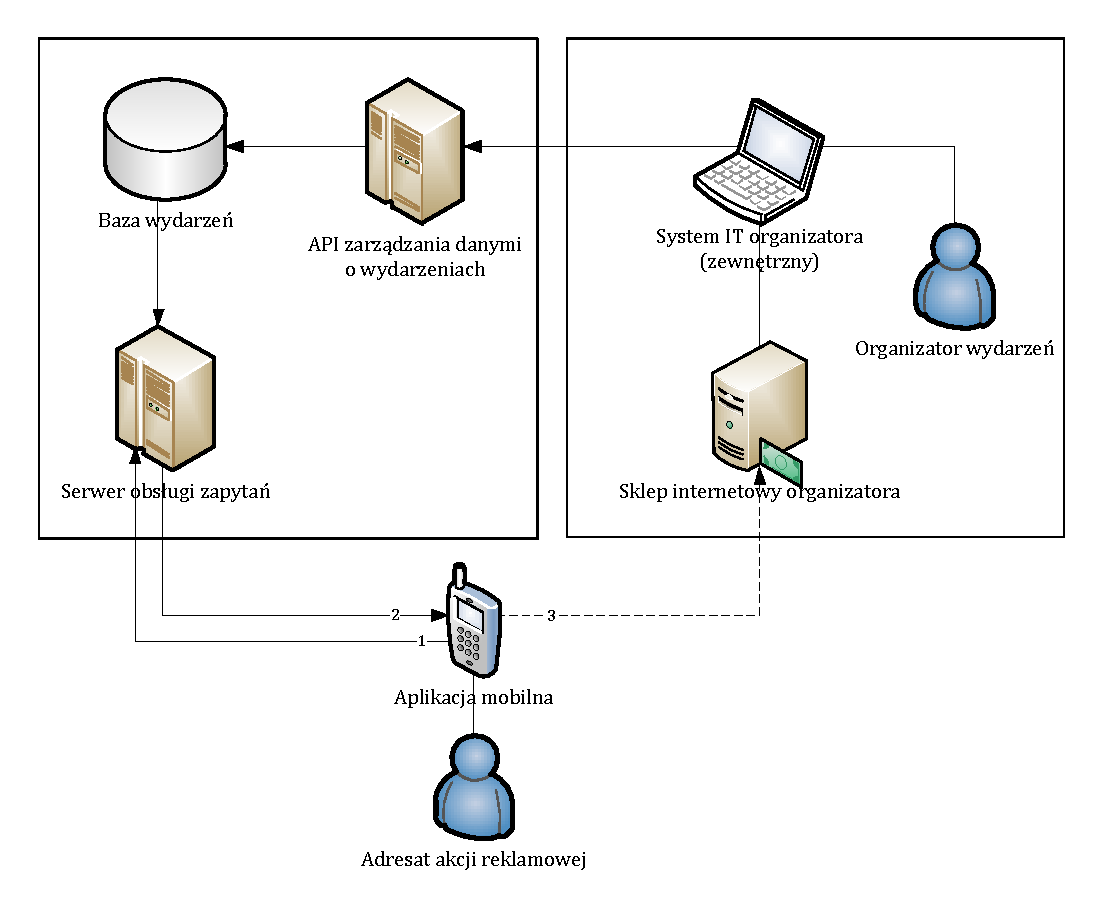
\includegraphics[width=\textwidth]{./figury/schemat-komponentow}
    \caption{Schemat współpracy wszystkich komponentów produktu.}
    \label{fig:schemat_komponentow}
\end{figure}


\newpage
\section*{Historia dokumentu}
\begin{versions}
    \version*{0.1}{2012-11-05}{TC}%
        Dodano \emph{Kontekst} i \emph{Opis produktu}.
    \version{0.2}{2012-11-06}{TC}%
        Dodano \emph{Wyzwania}.
    \version{0.3}{2012-11-08}{TC}%
        Zmieniono \emph{Cel projektu}.
    \version{0.3.1}{2012-11-09}{MO}%
        Ujednolicono terminologię. Sprecyzowano \emph{Cel projektu}.
    \version{1.0.rc}{2012-11-09}{MM}%
        Sprawdzono.
    \version{1.0}{2012-11-09}{TC}%
        Zatwierdzono.
    \version{1.1}{2012-11-10}{TC}%
        Przeniesiono \emph{Cel projektu} i \emph{Wyzwania} do statutu projektu.
    \version{1.2}{2012-11-10}{TC}%
        Dodano załącznik ze schematem komponentów.
    \version{1.3}{2012-12-27}{TC}%
        Przekonwertowano do aktualnego formatu dokumentów.
    \version{1.4}{2012-12-27}{TC}%
        Poprawiono szczegóły w opisach komponentów systemu.
    \version{2.0}{2012-12-27}{TC}%
        Sprawdzono i zatwierdzono.
\end{versions}


\end{document}
